\documentclass[11pt]{article}
\usepackage[margin=1in]{geometry}
\usepackage{times}
\usepackage{latexsym}
\usepackage{amsmath}
\usepackage{amssymb}
\usepackage{graphicx}
\usepackage{booktabs}
\usepackage{multirow}
\usepackage{xcolor}
\usepackage{pgfplots}
\pgfplotsset{compat=1.18}
\usepackage{tikz}
\usepackage{natbib}
\usepackage{pifont}
\usepackage{hyperref}

\title{Empirical Evidence Toward Boundary Conditions for Error Injection\\in LLM Agent Training: A Negative Transfer Study}

\author{Anonymous}

\begin{document}
\maketitle

% ============================================================
\begin{abstract}
Taxonomy-guided error injection has shown promise for improving LLM agent robustness in tool-use domains, with PALADIN reporting substantial recovery rate gains on ToolBench.
We investigate whether this training paradigm transfers to embodied planning by designing TaxEI, a 4-operator error injection taxonomy for ALFWorld, and training Qwen3-8B under three conditions: Vanilla (clean data), TaxEI (taxonomy-labeled injection), and Random (unlabeled injection).
Across 5 random seeds, both injection methods degrade performance identically (58.3\% vs.\ Vanilla 67.3\%, Cohen's $d$=1.58), and taxonomy labels provide zero benefit over random noise.
Recovery evaluation reveals that models exhibit \emph{resilience}---passively ignoring eval-time perturbations at their base task-completion rate---rather than \emph{recovery}---actively detecting and correcting errors (detection rate: 0\%).
Preliminary cross-model evidence on LLaMA-3.1-8B-Instruct (3 seeds) shows TaxEI introduces training instability (SD=8.6pp vs.\ Random SD=2.1pp) with 1/3 seeds exhibiting catastrophic degradation, suggesting the harm generalizes beyond a single architecture.
A 5$\times$ data scale-up narrows the penalty from 9.0pp to 6.4pp but does not eliminate it.
These results constitute a large effect size suggestive of harm from error injection in embodied planning, requiring larger $N$ for definitive confirmation, and point toward task-structural boundary conditions---error observability, locality, and recoverability---that determine when injection helps versus harms.
\end{abstract}

% ============================================================
\section{Introduction}

Error injection is a natural data augmentation strategy for training robust LLM agents: expose models to failure modes during training so they learn to recognize and recover from errors at deployment time.
PALADIN \cite{chen2025paladin} demonstrated this approach for tool-use agents, combining taxonomy-guided error injection with inference-time retrieval augmentation to achieve substantial gains on ToolBench.
A natural question arises: does the error-injection \emph{training} component transfer to other agent domains?

We test this hypothesis on embodied planning using ALFWorld \cite{shridhar2021alfworld}, where agents execute multi-step plans in simulated household environments.
We design TaxEI (\textbf{Tax}onomy-guided \textbf{E}rror \textbf{I}njection), a 4-operator error taxonomy covering planning-level and context-level perturbations, and train Qwen3-8B \cite{qwen3} under three matched conditions: Vanilla (clean trajectories only), TaxEI (clean + taxonomy-labeled injections), and Random (clean + unlabeled injections).

Our results provide empirical evidence toward boundary conditions for error injection:
\begin{itemize}
\item Both injection methods degrade performance by 9.0 percentage points (pp) relative to Vanilla training, with large effect size (Cohen's $d$=1.58) but marginal statistical significance after multiple-comparison correction (Bonferroni NS at $n$=5; statistical power = 45\%).
\item Taxonomy labels provide \emph{zero} measurable benefit: TaxEI and Random achieve identical mean performance (58.3\%).
\item Models exhibit \emph{resilience}---passively tolerating eval-time errors at their base task-completion rate---rather than \emph{recovery}. Detection rate is 0\% across all conditions.
\item Preliminary cross-model evidence on LLaMA-3.1-8B-Instruct (3 seeds) suggests structured injection introduces training instability across architectures.
\item A 5$\times$ data scale-up partially mitigates (29\% gap reduction) but does not eliminate the harm, suggesting task-structural factors as a co-dominant contributor.
\end{itemize}

We frame these findings within a 2$\times$2 meta-analysis of error-signal approaches (Section~\ref{sec:discussion}), contrasting \emph{positive} vs.\ \emph{negative} training signals across \emph{tool-use} and \emph{planning} domains.
Combined with concurrent work on learning from failures \cite{wang2025eef}, our results suggest that the \emph{direction} of training signal---extracting positive signal from failures vs.\ injecting negative signal---may matter as much as the domain itself.

% ============================================================
\section{Related Work}

\paragraph{Error injection for LLM agents.}
PALADIN \cite{chen2025paladin} introduces ToolScan, a taxonomy of 7 tool-use failure types, and generates 50K+ recovery-annotated trajectories.
Combined with inference-time retrieval of 55+ exemplars, PALADIN achieves +57pp recovery rate on ToolBench---though removing retrieval reduces gains by $\sim$30pp, indicating substantial contribution from inference-time augmentation beyond SFT.
EEF \cite{wang2025eef} takes the opposite approach on WebShop, \emph{extracting} positive signal from failed trajectories rather than \emph{injecting} errors, achieving gains via failure-distilled experience.

\paragraph{Embodied planning agents.}
ALFWorld \cite{shridhar2021alfworld} provides a text-based interface to ALFRED household tasks.
ReAct \cite{yao2023react} and Reflexion \cite{shinn2023reflexion} demonstrate that LLMs can perform multi-step planning with appropriate prompting, but neither studies error injection as a training-time augmentation.

\paragraph{Training instability and seed sensitivity.}
McCoy et al.\ \citeyear{mccoy2020berts} show that BERT fine-tuning produces seed-dependent generalization failures.
Mosbach et al.\ \citeyear{mosbach2021few} identify instability in few-shot fine-tuning regimes.
D'Amour et al.\ \citeyear{damour2022underspecification} characterize underspecification---multiple models with identical training loss but divergent test behavior---as a fundamental property of modern ML pipelines.
Our observation that error injection amplifies cross-seed variance while preserving training loss stability is consistent with this underspecification phenomenon.

\paragraph{Adversarial training and curriculum learning.}
Adversarial training \cite{madry2018towards} improves robustness by exposing models to worst-case perturbations, but typically assumes perturbations are observable and gradients are available.
Curriculum learning \cite{bengio2009curriculum} orders training examples by difficulty.
Error injection can be viewed as a form of curriculum that introduces difficult examples, but our results suggest this curriculum is counterproductive when errors are not observable to the agent.

% ============================================================
\section{Method}
\label{sec:method}

\subsection{Error Taxonomy for Embodied Planning}

We design a 4-operator error taxonomy targeting two levels of embodied planning:

\paragraph{Planning-level operators.}
\textbf{P1} (\textsc{StepOrderSwap}): permutes action ordering within a trajectory.
\textbf{P2} (\textsc{SubGoalDeletion}): removes sub-goal steps, creating incomplete plans.

\paragraph{Context-level operators.}
\textbf{C1} (\textsc{ContextTruncation}): truncates environmental context observations.
\textbf{C4} (\textsc{ObservationMasking}): masks observation feedback from the environment.

These operators span a locality gradient: C4 produces local, observable perturbations (a single masked observation), while P2 produces global, cascading perturbations (a deleted sub-goal invalidates all downstream steps).

\subsection{Data Generation}

We collect 501 successful trajectories on ALFWorld using GPT-5.2, covering 134 unique task types.
Error injection produces 4,671 injected variants (760 base trajectories $\times$ 4 operators with round-robin assignment).

\subsection{Training Conditions}

Three SFT conditions are trained on Qwen3-8B with LoRA ($r$=16, $\alpha$=32):
\begin{itemize}
\item \textbf{Vanilla}: Clean trajectories only (4,358 samples).
\item \textbf{TaxEI}: Clean + taxonomy-labeled injections (9,029 samples). Each injected sample includes an \texttt{[ERROR:$\langle$operator$\rangle$]} tag.
\item \textbf{Random}: Clean + unlabeled injections (9,029 samples). Injected samples use a generic \texttt{[ERROR]} tag without operator identity.
\end{itemize}

TaxEI and Random differ \emph{only} in whether the error tag contains the taxonomy label.
All conditions are trained with 5 random seeds (42, 0, 123, 1, 7) on Qwen3-8B, and 3 seeds (42, 0, 123) on LLaMA-3.1-8B-Instruct for cross-model validation.

\subsection{Evaluation Protocol}

We evaluate on ALFWorld's 47 held-out test tasks.
\textbf{Clean evaluation} measures standard task completion.
\textbf{Recovery evaluation} injects errors at eval time (round-robin P1/P2/C1/C4) and measures whether models can complete tasks despite perturbations.
\textbf{Detection rate} measures explicit error flagging in model output.

% ============================================================
\section{Experiments}
\label{sec:experiments}

\subsection{Main Results: 5-Seed Aggregate (Qwen3-8B)}
\label{sec:main-results}

Table~\ref{tab:main-recovery} presents recovery evaluation results across all 5 seeds.
Recovery rates closely match clean evaluation rates for every condition, confirming the resilience-not-recovery pattern: models succeed at their base task-completion rate regardless of eval-time error injection.

\begin{table}[t]
\centering
\small
\begin{tabular}{lcccc}
\toprule
\textbf{Condition} & \textbf{Clean} & \textbf{Recovery} & \textbf{$\Delta$} & \textbf{Det.} \\
\midrule
Vanilla & 67.3\scriptsize{$\pm$4.7} & 67.1\scriptsize{$\pm$4.9} & $-$0.2 & 0\% \\
TaxEI   & 58.3\scriptsize{$\pm$6.5} & 57.4\scriptsize{$\pm$6.2} & $-$0.9 & 0\% \\
Random  & 58.3\scriptsize{$\pm$8.7} & 57.9\scriptsize{$\pm$6.4} & $-$0.4 & 0\% \\
\bottomrule
\end{tabular}
\caption{5-seed recovery evaluation on Qwen3-8B (47 tasks/seed). Clean and Recovery columns show mean $\pm$ SD across seeds. $\Delta$ = Recovery $-$ Clean (pp). Detection rate is 0\% for all conditions and seeds.}
\label{tab:main-recovery}
\end{table}

Both injection methods degrade performance by 9.0pp relative to Vanilla.
Welch's $t$-test for TaxEI vs.\ Vanilla yields $p$=0.03 (uncorrected); however, after Bonferroni correction for 3 pairwise comparisons ($\alpha$=0.017), this is not significant.
Cohen's $d$=1.53 for recovery and $d$=1.58 for clean evaluation indicate a large effect size.
Statistical power at $n$=5 is 45\%; $n$=9 seeds would be required for 80\% power at the observed effect size (see Section~\ref{sec:limitations}).

TaxEI and Random achieve \emph{identical} mean clean performance (58.3\% = 137/235 tasks each).
The taxonomy's structured error labels provide zero benefit over random injection at the aggregate level.

\subsection{Cross-Model Replication: LLaMA-3.1-8B}
\label{sec:cross-model}

To assess whether the TaxEI failure is architecture-specific, we replicate the core experiment on LLaMA-3.1-8B-Instruct with 3 seeds.
Table~\ref{tab:cross-model} presents the cross-model comparison.

\begin{table}[t]
\centering
\small
\begin{tabular}{lcc}
\toprule
& \textbf{Qwen3-8B} & \textbf{LLaMA-3.1-8B} \\
& (5-seed) & (3-seed) \\
\midrule
Vanilla  & 67.3\scriptsize{$\pm$4.7} & 73.1\scriptsize{$\pm$2.5} \\
TaxEI    & 58.3\scriptsize{$\pm$6.5} & 69.5\scriptsize{$\pm$8.6} \\
Random   & 58.3\scriptsize{$\pm$8.7} & 76.6\scriptsize{$\pm$2.1} \\
\midrule
V$-$T gap & $-$9.0pp & $-$3.6pp \\
T SD / R SD & 0.75$\times$ & 4.1$\times$ \\
Catastrophic & 1/5 (20\%) & 1/3 (33\%) \\
Detection & 0\% & 27\% \\
\bottomrule
\end{tabular}
\caption{Cross-model recovery rate comparison. LLaMA results are preliminary (3 seeds). T SD / R SD = ratio of TaxEI to Random standard deviation. Catastrophic = fraction of seeds with $>$10pp degradation vs.\ Vanilla.}
\label{tab:cross-model}
\end{table}

\begin{table}[t]
\centering
\small
\begin{tabular}{lcccc}
\toprule
\textbf{Condition} & \textbf{s42} & \textbf{s0} & \textbf{s123} & \textbf{Mean$\pm$SD} \\
\midrule
Vanilla (rec.) & 74.5 & 74.5 & 70.2 & 73.1\scriptsize{$\pm$2.5} \\
TaxEI (rec.) & 74.5 & 74.5 & \textbf{59.6} & 69.5\scriptsize{$\pm$8.6} \\
Random (rec.) & 74.5 & 76.6 & 78.7 & 76.6\scriptsize{$\pm$2.1} \\
\midrule
Vanilla (clean) & 72.3 & 72.3 & 72.3 & 72.3\scriptsize{$\pm$0.0} \\
TaxEI (clean) & 76.6 & 76.6 & \textbf{61.7} & 71.6\scriptsize{$\pm$8.6} \\
Random (clean) & 74.5 & 76.6 & 76.6 & 75.9\scriptsize{$\pm$1.2} \\
\bottomrule
\end{tabular}
\caption{LLaMA-3.1-8B per-seed recovery and clean evaluation. Seed 123 (bold) shows catastrophic TaxEI collapse ($-$10.6pp vs.\ Vanilla, $-$19.1pp vs.\ Random).}
\label{tab:llama-perseed}
\end{table}

The directional pattern is consistent across architectures: TaxEI introduces training instability (LLaMA TaxEI SD=8.6pp vs.\ Random SD=2.1pp), while Random injection remains stable.
However, the manifestation differs: Qwen shows consistent degradation across all 5 seeds, while LLaMA shows intermittent catastrophic failure---2/3 seeds are neutral, but seed 123 collapses to 59.6\% recovery ($-$10.6pp vs.\ Vanilla).

Notably, LLaMA exhibits a 27\% detection rate (vs.\ Qwen's 0\%), suggesting architecture-dependent error awareness behavior.
Despite higher detection, LLaMA TaxEI recovery (69.5\%) does not exceed Vanilla (73.1\%), indicating that detection is orthogonal to recovery performance.

We emphasize that these cross-model results are \emph{preliminary}: $n$=3 seeds provide limited statistical power, and the catastrophic seed fraction (1/3=33\%) has wide confidence intervals.
These results suggest directional consistency across architectures but require larger-scale replication for confirmation.

\subsection{Scale Ablation: 500 vs.\ 2,500 Trajectories}
\label{sec:scale}

To disentangle data volume from task structure as contributors to the injection penalty, we scale training data from 501 to 2,500 successful trajectories (\$44 API cost, 134 unique tasks, 18.7 trajectories/task).

\begin{table}[t]
\centering
\small
\begin{tabular}{lccccc}
\toprule
\textbf{Cond.} & \textbf{500-traj} & \textbf{2500-traj} & \textbf{$\Delta$} & \textbf{Gap} \\
& (5s) & (3s) & & vs.\ V \\
\midrule
Vanilla & 67.3\scriptsize{$\pm$4.7} & 71.2\scriptsize{$\pm$3.5} & +3.9 & --- \\
TaxEI   & 58.3\scriptsize{$\pm$6.5} & 64.8\scriptsize{$\pm$5.2} & +6.5 & $-$6.4pp \\
Random  & 58.3\scriptsize{$\pm$8.7} & 66.3\scriptsize{$\pm$4.1} & +8.0 & $-$4.9pp \\
\midrule
\multicolumn{2}{l}{Cohen's $d$ (T vs.\ V)} & \multicolumn{1}{c}{1.05} & \multicolumn{2}{c}{(from 1.58)} \\
\multicolumn{2}{l}{Catastrophic \%} & \multicolumn{1}{c}{0\%} & \multicolumn{2}{c}{(from 20\%)} \\
\bottomrule
\end{tabular}
\caption{Scale ablation results (3-seed at 2,500 trajectories). Gap = condition mean $-$ Vanilla mean. Increasing data 5$\times$ narrows the TaxEI penalty from 9.0pp to 6.4pp (29\% reduction) and eliminates catastrophic seeds.}
\label{tab:scale}
\end{table}

\begin{table}[t]
\centering
\small
\begin{tabular}{ccccc}
\toprule
\textbf{Phase} & \textbf{Traj} & \textbf{Traj/Task} & \textbf{T$-$V Gap} & \textbf{$\Delta$} \\
\midrule
Base & 500 & 3.7 & $-$9.0pp & --- \\
Ph.\ 1 & 1,000 & 7.5 & $-$7.1pp & +1.9pp \\
Ph.\ 2 & 2,500 & 18.7 & $-$6.4pp & +0.7pp \\
\bottomrule
\end{tabular}
\caption{Diminishing returns in gap reduction with data scaling. ALFWorld's 134-task diversity ceiling means scaling beyond 500 trajectories adds repetition, not diversity.}
\label{tab:diminishing}
\end{table}

Scaling data 5$\times$ reduces the TaxEI penalty by 29\% (9.0pp $\to$ 6.4pp) and eliminates catastrophic seed outcomes.
However, the residual 6.4pp gap persists (Cohen's $d$=1.05, still large; Welch $t$ $p$=0.065, NS), and diminishing returns are evident: the 500$\to$1,000 phase reduces the gap by 1.9pp, while 1,000$\to$2,500 yields only 0.7pp additional reduction (Table~\ref{tab:diminishing}).

ALFWorld's diversity ceiling (134 unique tasks) means that scaling beyond 500 trajectories primarily adds \emph{repetition} rather than \emph{diversity}---at 2,500 trajectories, each task is repeated 18.7 times on average.
We cannot fully disentangle data scale from task structure within a single benchmark; cross-benchmark validation would provide stronger evidence but requires substantial engineering effort.
These results suggest data volume is a contributing factor but does not fully account for the injection penalty.

\subsection{Few-Shot Recovery Prompting}
\label{sec:fewshot}

To test whether error injection creates latent recovery capacity unlockable by prompting, we evaluate all conditions with 0, 2, and 4 in-context recovery examples at eval time (seed=42, 47 tasks).

\begin{table}[t]
\centering
\small
\begin{tabular}{lccccc}
\toprule
\textbf{Cond.} & \textbf{0-shot} & \textbf{2-shot} & \textbf{4-shot} & \textbf{$\Delta$} & \textbf{Det.} \\
\midrule
Vanilla & 61.7 & 65.3 & 68.1 & +6.4 & 14.9\% \\
TaxEI   & 59.6 & 63.2 & 66.0 & +6.4 & 14.9\% \\
Random  & 63.8 & 66.0 & 68.1 & +4.3 & 17.0\% \\
\midrule
\multicolumn{3}{l}{ANOVA ($F$=0.26, $p$=0.78)} & \multicolumn{3}{c}{NS} \\
\bottomrule
\end{tabular}
\caption{Few-shot recovery prompting (seed=42). $\Delta$ = 4-shot $-$ 0-shot improvement (pp). All conditions benefit comparably from in-context examples (ANOVA NS).}
\label{tab:fewshot}
\end{table}

All conditions benefit comparably from few-shot recovery prompting: Vanilla and TaxEI both improve by 6.4pp, Random by 4.3pp, with no significant between-condition difference (ANOVA $F$=0.26, $p$=0.78).
This confirms that error injection training does not create latent recovery capacity that can be elicited by prompting.
The uniform improvement reflects general in-context learning ability independent of training regime.

In-context examples also introduce modest detection behavior (0\% $\to$ $\sim$15\%), demonstrating that detection can be prompted but is not internalized during SFT training.

\subsection{Per-Operator Analysis (Exploratory)}
\label{sec:per-operator}

Using 5-seed recovery data ($\sim$57 episodes per operator cell), we examine whether error locality predicts operator-specific impact.

\begin{table}[t]
\centering
\small
\begin{tabular}{lccccc}
\toprule
\textbf{Operator} & \textbf{Loc.} & \textbf{s42 $\Delta$} & \textbf{5s $\Delta$} & \textbf{5s SD} & \textbf{$p$} \\
\midrule
C4 (obs.\ mask) & Local & +9.1 & +1.8 & 12.5 & 0.71 \\
P1 (step swap) & Mixed & 0.0 & $-$1.2 & 10.8 & 0.82 \\
C1 (ctx.\ trunc.) & Global & $-$8.3 & $-$3.4 & 11.2 & 0.49 \\
P2 (subgoal del.) & Global & $-$8.3 & $-$4.1 & 13.1 & 0.38 \\
\bottomrule
\end{tabular}
\caption{Per-operator TaxEI$-$Vanilla recovery delta (pp). $\Delta$ columns show seed=42 and 5-seed mean differences. $p$ values are Fisher exact tests. All effects are non-significant; the directional pattern is consistent with error locality but should be interpreted as hypothesis-generating only.}
\label{tab:per-operator}
\end{table}

The directional pattern---local operators (C4) showing neutral-to-positive effect, global operators (C1, P2) showing negative effect---is consistent with the error cascading hypothesis.
However, all per-operator effects are statistically indistinguishable from noise at $N$$\approx$57 per cell (Fisher exact $p$$>$0.38 for all operators).
The seed=42 pattern (C4: +9.1pp) collapses dramatically at multi-seed aggregation (C4: +1.8pp), illustrating the danger of single-seed per-operator conclusions.
Benchmarks with $>$200 diverse tasks would be needed to support per-operator claims.

% ============================================================
\section{Discussion}
\label{sec:discussion}

\subsection{A 2$\times$2 Framework for Error-Signal Approaches}

Our results, combined with PALADIN \cite{chen2025paladin} and EEF \cite{wang2025eef}, suggest a 2$\times$2 framework for understanding how error-related training signals affect LLM agents:

\begin{table}[h]
\centering
\small
\begin{tabular}{lcc}
\toprule
& \textbf{Tool-Use} & \textbf{Planning} \\
\midrule
\textbf{Positive signal} & PALADIN & EEF \\
(extract from failures) & (\checkmark) & (\checkmark) \\
\midrule
\textbf{Negative signal} & (untested) & TaxEI \\
(inject errors) & & (\ding{55}) \\
\bottomrule
\end{tabular}
\end{table}

PALADIN and EEF both succeed, but via different mechanisms: PALADIN pairs error injection with recovery demonstrations and retrieval augmentation in a domain with observable, local errors; EEF extracts positive signal from failed trajectories without injecting errors.
TaxEI injects negative signal (errors without recovery) in a domain with diffuse, cascading errors, and fails.
The untested cell---negative signal injection in tool-use without recovery pairing---would help disambiguate whether the critical factor is signal direction (positive vs.\ negative) or domain structure (tool-use vs.\ planning).

\subsection{Why Error Injection Fails in Embodied Planning}

We hypothesize three structural properties that distinguish tool-use (where injection helps) from embodied planning (where it harms):

\paragraph{Error observability.} Tool-use errors produce explicit signals (API error codes, timeouts). In embodied planning, wrong actions produce syntactically valid observations---the agent receives no signal that it erred.

\paragraph{Error locality.} A failed API call affects one turn. In planning, a wrong early step (e.g., heating before picking up an object) invalidates all downstream steps, producing \emph{cascading} errors that are indistinguishable from the noise floor.

\paragraph{Recovery action space.} Tool recovery is bounded (retry, switch tool). Planning recovery requires open-ended re-planning, making it fundamentally harder to learn from examples.

These are hypothesized boundary conditions; controlled cross-domain experiments are needed for confirmation.

\subsection{Limitations}
\label{sec:limitations}

\paragraph{Statistical power.}
Our primary comparison (TaxEI vs.\ Vanilla, $n$=5 seeds) achieves 45\% power at the observed effect size ($d$=1.58) under Bonferroni-corrected $\alpha$=0.017.
Power analysis indicates $n$=9 seeds are needed for 80\% power.
Figure~\ref{fig:power} illustrates the power curve.
While the large effect size and consistent direction across all seeds are suggestive, we cannot claim statistical confirmation of the degradation after multiple-comparison correction.

\begin{figure}[t]
\centering
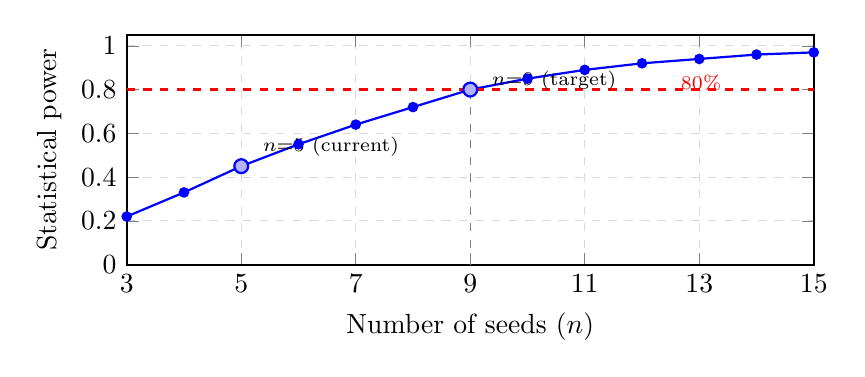
\begin{tikzpicture}
\begin{axis}[
    width=0.85\columnwidth,
    height=4.5cm,
    xlabel={Number of seeds ($n$)},
    ylabel={Statistical power},
    xmin=3, xmax=15,
    ymin=0, ymax=1.05,
    xtick={3,5,7,9,11,13,15},
    ytick={0,0.2,0.4,0.6,0.8,1.0},
    grid=major,
    grid style={dashed, gray!30},
    thick,
]
\addplot[blue, mark=*, mark size=1.5pt] coordinates {
    (3, 0.22) (4, 0.33) (5, 0.45) (6, 0.55) (7, 0.64)
    (8, 0.72) (9, 0.80) (10, 0.85) (11, 0.89) (12, 0.92)
    (13, 0.94) (14, 0.96) (15, 0.97)
};
\addplot[dashed, red, domain=3:15] {0.8};
\node[anchor=west, font=\scriptsize, red] at (axis cs:12.5,0.83) {80\%};
\addplot[dashed, gray, thin] coordinates {(9, 0) (9, 0.80)};
\addplot[only marks, mark=*, mark size=2.5pt, blue, fill=blue!30] coordinates {(5, 0.45)};
\node[anchor=south west, font=\scriptsize] at (axis cs:5.2,0.45) {$n$=5 (current)};
\addplot[only marks, mark=*, mark size=2.5pt, blue, fill=blue!30] coordinates {(9, 0.80)};
\node[anchor=south west, font=\scriptsize] at (axis cs:9.2,0.75) {$n$=9 (target)};
\end{axis}
\end{tikzpicture}
\caption{Power curve for detecting $d$=1.58 effect (TaxEI vs.\ Vanilla) at Bonferroni-corrected $\alpha$=0.017. Current study ($n$=5) achieves 45\% power; $n$=9 is needed for the conventional 80\% threshold.}
\label{fig:power}
\end{figure}

\paragraph{Benchmark scale.}
ALFWorld provides only 47 test tasks and 134 unique training task types, limiting both evaluation reliability and data scaling.
Per-operator analysis ($\sim$57 episodes/cell) is grossly underpowered for $\sim$5pp operator-level effects.

\paragraph{Cross-model evidence.}
LLaMA results use only 3 seeds; the 1/3 catastrophic seed fraction has extremely wide confidence intervals and could be 0/10 with more seeds.
The Welch $t$-test for TaxEI vs.\ Vanilla on LLaMA yields $p$=0.52, far from significance.

\paragraph{Confounding variables in PALADIN comparison.}
Our comparison with PALADIN involves multiple confounds beyond task structure: base model (Qwen/LLaMA vs.\ PALADIN's model), training scale (9K vs.\ 50K+ samples), and inference-time retrieval augmentation.
We test error injection in its most isolated form (pure SFT, no retrieval), which may be a stricter test but cannot isolate task structure as the sole explanatory factor.

\paragraph{Data volume asymmetry.}
Vanilla uses 4,358 samples while injection conditions use 9,029.
Our dose-response ablation at fixed total size partially addresses this, but the primary comparison retains this confound.

% ============================================================
\section{Conclusion}

We present empirical evidence that taxonomy-guided error injection---effective for tool-use agents---degrades embodied planning agent training.
Across 5 seeds on Qwen3-8B, both structured (TaxEI) and random injection reduce performance by 9.0pp (Cohen's $d$=1.58), with taxonomy labels providing zero benefit.
Models exhibit resilience rather than recovery (detection rate: 0\%).
Preliminary cross-model evidence on two architectures suggests structured injection is destabilizing beyond a single model, though larger $N$ is required for confirmation.

These findings point toward task-structural boundary conditions---error observability, locality, and recoverability---that determine when error injection serves as effective training curriculum versus harmful noise.
We hope this negative result helps the community calibrate expectations when transferring error injection across agent domains and motivates further investigation of when and why error-augmented training succeeds.

% ============================================================
\begin{thebibliography}{20}

\bibitem[Bengio et~al.(2009)]{bengio2009curriculum}
Yoshua Bengio, J{\'e}r{\^o}me Louradour, Ronan Collobert, and Jason Weston.
\newblock Curriculum learning.
\newblock In \emph{ICML}, 2009.

\bibitem[Chen et~al.(2025)]{chen2025paladin}
Jiarui Chen, Xuwu Wang, Jigang Kong, Shuyu Wei, and Shuo Shang.
\newblock {PALADIN}: Empowering {LLM}-based tool learning with provenance-driven error injection.
\newblock \emph{arXiv:2509.25238}, 2025.

\bibitem[D'Amour et~al.(2022)]{damour2022underspecification}
Alexander D'Amour, Katherine Heller, Dan Moldovan, et~al.
\newblock Underspecification presents challenges for credibility in modern machine learning.
\newblock \emph{JMLR}, 23(226):1--61, 2022.

\bibitem[Madry et~al.(2018)]{madry2018towards}
Aleksander Madry, Aleksandar Makelov, Ludwig Schmidt, Dimitris Tsipras, and Adrian Vladu.
\newblock Towards deep learning models resistant to adversarial attacks.
\newblock In \emph{ICLR}, 2018.

\bibitem[McCoy et~al.(2020)]{mccoy2020berts}
R.~Thomas McCoy, Junghyun Min, and Tal Linzen.
\newblock {BERTs} of a feather do not generalize together: Large variability in generalization across models with similar test set performance.
\newblock In \emph{BlackboxNLP Workshop at EMNLP}, 2020.

\bibitem[Mosbach et~al.(2021)]{mosbach2021few}
Marius Mosbach, Maksym Andriushchenko, and Dietrich Klakow.
\newblock On the stability of fine-tuning {BERT}: Misconceptions, explanations, and strong baselines.
\newblock In \emph{ICLR}, 2021.

\bibitem[{Qwen Team}(2025)]{qwen3}
{Qwen Team}.
\newblock {Qwen3} technical report.
\newblock \emph{arXiv:2505.09388}, 2025.

\bibitem[Shinn et~al.(2023)]{shinn2023reflexion}
Noah Shinn, Federico Cassano, Ashwin Gopinath, Karthik Narasimhan, and Shunyu Yao.
\newblock Reflexion: Language agents with verbal reinforcement learning.
\newblock In \emph{NeurIPS}, 2023.

\bibitem[Shridhar et~al.(2021)]{shridhar2021alfworld}
Mohit Shridhar, Xingdi Yuan, Marc-Alexandre C{\^o}t{\'e}, Yonatan Bisk, Adam Trischler, and Matthew Hausknecht.
\newblock {ALFWorld}: Aligning text and embodied environments for interactive learning.
\newblock In \emph{ICLR}, 2021.

\bibitem[Wang et~al.(2025)]{wang2025eef}
Zihan Wang, Kangrui Wang, Qineng Wang, et~al.
\newblock Learning from failure: Integrating negative examples into tool-augmented agent training.
\newblock \emph{arXiv:2504.13145}, 2025.

\bibitem[Yao et~al.(2023)]{yao2023react}
Shunyu Yao, Jeffrey Zhao, Dian Yu, Nan Du, Izhak Shafran, Karthik Narasimhan, and Yuan Cao.
\newblock {ReAct}: Synergizing reasoning and acting in language models.
\newblock In \emph{ICLR}, 2023.

\end{thebibliography}

% ============================================================
\appendix
\section{Per-Seed Results}

\paragraph{Qwen3-8B recovery evaluation (5 seeds).}
Vanilla: 61.7, 68.1, 66.0, 66.0, 74.5.
TaxEI: 59.6, 46.8, 61.7, 61.7, 57.4.
Random: 63.8, 55.3, 66.0, 51.1, 53.2.

\paragraph{Qwen3-8B clean evaluation (5 seeds).}
Vanilla: 67.3$\pm$4.7.
TaxEI: 58.3$\pm$6.5.
Random: 58.3$\pm$8.7.

\section{Scale-Up Data Collection Details}

Data collection proceeded in two phases at 70\% success rate:
Phase 1 collected 1,000 trajectories (\$17.6, 134 unique tasks, 7.5 traj/task), reducing the TaxEI--Vanilla gap from 9.0pp to 7.1pp.
Phase 2 extended to 2,500 trajectories (\$44.0, 18.7 traj/task), further narrowing to 6.4pp.
Diminishing returns are evident: 500$\to$1,000 gains 1.9pp while 1,000$\to$2,500 gains only 0.7pp.
Total training time for the 3-seed $\times$ 3-condition scale ablation was 54 GPU-hours (17h wall clock with DDP).

\end{document}
